
\bta{2014}


\section{ Use of English}

\textbf{Directions:}\\
 Read the following text. Choose the best word (s) for
	each numbered blank and mark A, B, C or D on \textbf{ANSWER SHEET 1}. (10
	points)



\TiGanSpace



As many people hit middle age, they often start to notice that their
memory and mental clarity are not what they used to be. We suddenly
can't remember \cloze we put the keys just a moment ago, or an
old acquaintance's name, or the name of an old band we used to love. As
the brain \cloze , we refer to these occurrences as " senior
moments." \cloze seemingly innocent, this loss of mental focus
can potentially have a(an) \cloze impact on our professional,
social, and personal \cloze.

Neuroscientists, experts who study the nervous system, are increasingly
showing that there's actually a lot that can be done. It \cloze
out that the brain needs exercise in much the same way our muscles do,
and the right mental \cloze can significantly improve our basic
cognitive \cloze. Thinking is essentially a \cloze of
making connections in the brain. To a certain extent, our ability to
\cloze in making the connections that drive intelligence is
inherited. \cloze , because these connections are made through
effort and practice, scientists believe that intelligence can expand and
fluctuate \cloze mental effort.

Now, a new Web-based company has taken it a step \cloze and
developed the first ``brain training program'' designed to actually help
people improve and regain their mental \cloze.

The Web-based program \cloze you to systematically improve your
memory and attention skills. The program keeps \cloze of your
progress and provides detailed feedback \cloze your performance
and improvement. Most importantly, it \cloze modifies and
enhances the games you play to \cloze on the strengths you are
developing--much like a(n) \cloze exercise routine requires
you to increase resistance and vary your muscle use.


\newpage

\begin{enumerate}
	%\renewcommand{\labelenumi}{\arabic{enumi}.}
	% A(\Alph) a(\alph) I(\Roman) i(\roman) 1(\arabic)
	%设定全局标号series=example	%引用全局变量resume=example
	%[topsep=-0.3em,parsep=-0.3em,itemsep=-0.3em,partopsep=-0.3em]
	%可使用leftmargin调整列表环境左边的空白长度 [leftmargin=0em]
	\item


\fourchoices
{why}
{when}
{that}
{where}




\item


\fourchoices
{improves}
{fades}
{collapses}
{recovers}




\item


\fourchoices
{While}
{Unless}
{Once}
{If}




\item


\fourchoices
{uneven}
{limited}
{damaging}
{obscure}




\item

\fourchoices
{relationship}
{environment}
{wellbeing}
{outlook}



\item


\fourchoices
{turns}
{finds}
{points}
{figures}




\item

\fourchoices
{responses}
{roundabouts}
{workouts}
{associations}



\item

\fourchoices
{genre}
{criterion}
{circumstances}
{functions}



\item


\fourchoices
{channel}
{process}
{sequence}
{condition}




\item


\fourchoices
{excel}
{feature}
{persist}
{believe}




\item


\fourchoices
{However}
{Moreover}
{Otherwise}
{Therefore}




\item

\fourchoices
{instead of}
{regardless of}
{apart from}
{according to}


\item


\fourchoices
{back}
{further}
{aside}
{around}




\item

\fourchoices
{framework}
{stability}
{sharpness}
{flexibility}


\item


\fourchoices
{hurries}
{reminds}
{forces}
{allows}




\item


\fourchoices
{order}
{track}
{hold}
{pace}




\item


\fourchoices
{to}
{on}
{for}
{with}




\item

\fourchoices
{constantly}
{habitually}
{irregularly}
{unusually}



\item


\fourchoices
{carry}
{put}
{build}
{take}




\item


\fourchoices
{risky}
{familiar}
{idle}
{effective}

\end{enumerate}


\vfil

\section{Reading Comprehension}


\noindent
\textbf{Part A}\\
\textbf{Directions:}\\
 Read the following four texts. Answer the questions
	after each text by choosing A, B, C or
	D. Mark your answers on \textbf{ANSWER SHEET 1}. (40 points)

\newpage
\subsection{Text 1}


In order to ``change lives for the better'' and reduce ``dependency,''
George Osbome, Chancellor of the Exchequer, introduced the ``upfront
work search'' scheme. Only if the jobless arrive at the jobcentre with
a CV, register for online job search, and start looking for work will
they be eligible for benefit---and then they should report weekly rather
than fortnightly. What could be more reasonable?

More apparent reasonableness followed. There will now be a seven-day
wait for the jobseeker's allowance. ``Those first few days should be
spent looking for work, not looking  \uline{to sign on},'' he
claimed. ``We're doing these things because we know they help people stay
off benefits and help those on benefits get into work faster.'' Help?
Really? On first hearing, this was the socially concerned chancellor,
trying to change lives for the better, complete with ``reforms'' to an
obviously indulgent system that demands too little effort from the newly
unemployed to find work, and subsidises laziness. What motivated him, we
were to understand, was his zeal for ``fundamental fairness''---protecting
the taxpayer, controlling spending and ensuring that only the most
deserving claimants received their benefits.

Losing a job is hurting: you don't skip down to the jobcentre with a
song in your heart, delighted at the prospect of doubling your income
from the generous state. It is financially terrifying, psychologically
embarrassing and you know that support is minimal and extraordinarily
hard to get. You are now not wanted; you support is minimal and
extraordinarily hard to get. You are now not wanted; you are now
excluded from the work environment that offers purpose and structure in
your life. Worse, the crucial income to feed yourself and your family
and pay the bills has disappeared. Ask anyone newly unemployed what they
want and the answer is always: a job.

But in Osborneland, your first instinct is to fall into dependency---permanent dependency if you can get it---supported by a state only too
ready to indulge your falsehood. It is as though 20 years of ever-tougher reforms of the job search and benefit administration system
never happened. The principle of British welfare is no longer that you
can insure yourself against the risk of unemployment and receive
unconditional payments if the disaster happens. Even the very phrase
``jobseeker's allowance'' is about redefining the
unemployed as a ``jobseeker'' who had no fundamental right to a benefit he
or she has earned through making national insurance contributions.
Instead, the claimant receives a time-limited ``allowance,'' conditional
on actively seeking a job; no entitlement and no insurance, at £71.70 a
week, one of the least generous in the EU.


\begin{enumerate}[resume]
	%\renewcommand{\labelenumi}{\arabic{enumi}.}
	% A(\Alph) a(\alph) I(\Roman) i(\roman) 1(\arabic)
	%设定全局标号series=example	%引用全局变量resume=example
	%[topsep=-0.3em,parsep=-0.3em,itemsep=-0.3em,partopsep=-0.3em]
	%可使用leftmargin调整列表环境左边的空白长度 [leftmargin=0em]
	\item
George Osborne's scheme was intended to \lineread.


\fourchoices
{provide the unemployed with easier access to benefits}
{encourage jobseekers' active engagement in job seeking}
{motivate the unemployed to report voluntarily}
{guarantee jobseekers' legitimate right to benefits}


\item
 The phrase ``to sign on'' (Line 3, Para. 2) most probably
means \lineread.


\fourchoices
{to check on the availability of jobs at the jobcentre}
{to accept the government's restrictions on the allowance}
{to register for an allowance from the government}
{to attend a governmental job-training program}



\item
What prompted the chancellor to develop his scheme?


\fourchoices
{A desire to secure a better life for all.}
{An eagerness to protect the unemployed.}
{An urge to be generous to the claimants.}
{A passion to ensure fairness for taxpayers.}


\item
According to Paragraph 3, being unemployed makes one feel \lineread.



\fourchoices
{uneasy}
{enraged}
{insulted}
{guilty}




\item
To which of the following would the author most probably
agree?


\fourchoices
{The British welfare system indulges jobseekers' laziness.}
{Osborne's reforms will reduce the risk of unemployment.}
{The jobseekers' allowance has met their actual needs.}
{Unemployment benefits should not be made conditional.}


\end{enumerate}



\newpage
\subsection{Text 2}


All around the world, lawyers generate more hostility than the members
of any other profession---with the possible exception of journalism.
But there are few places where clients have more grounds for complaint
than America.

During the decade before the economic crisis, spending on legal services
in America grew twice as fast as inflation. The best lawyers made
skyscrapers-full of money, tempting ever more students to pile into law
schools. But most law graduates never get a big-firm job. Many of them
instead become the kind of nuisance-lawsuit filer that makes the tort
system a costly nightmare.

There are many reasons for this. One is the excessive costs of a legal
education. There is just one path for a lawyer in most American states:
a four-year undergraduate degree in some unrelated subjects, then a
three-year law degree at one of 200 law schools authorized by the
American Bar Association and an expensive preparation for the bar exam.
This leaves today's average law-school graduate with \$100, 000 of debt
on top of undergraduate debts. Law-school debt means that they have to
work fearsomely hard.

Reforming the system would help both lawyers and their customers.
Sensible ideas have been around for a long time, but the state-level
bodies that govern the profession have been too conservative to
implement them. One idea is to allow people to study law as an
undergraduate degree. Another is to let students sit for the bar after
only two years of law school. If the bar exam is truly a stern enough
test for a would-be lawyer, those who can sit it earlier should be
allowed to do so. Students who do not need the extra training could cut
their debt mountain by a third.

The other reason why costs are so high is the restrictive guild-like
ownership structure of the business. Except in the District of Columbia,
non-lawyers may not own any share of a law firm. This keeps fees high
and innovation slow. There is pressure for change from within the
profession, but opponents of change among the regulators insist that
keeping outsiders out of a law firm isolates lawyers from the pressure
to make money rather than serve clients ethically.

In fact, allowing non-lawyers to own shares in law firms would reduce
costs and improve services to customers, by encouraging law firms to use
technology and to employ professional managers to focus on improving
firms' efficiency. After all, other countries, such as Australia and
Britain, have started liberalizing their legal professions. America
should follow.


\begin{enumerate}[resume]
	%\renewcommand{\labelenumi}{\arabic{enumi}.}
	% A(\Alph) a(\alph) I(\Roman) i(\roman) 1(\arabic)
	%设定全局标号series=example	%引用全局变量resume=example
	%[topsep=-0.3em,parsep=-0.3em,itemsep=-0.3em,partopsep=-0.3em]
	%可使用leftmargin调整列表环境左边的空白长度 [leftmargin=0em]
	\item
 A lot of students take up law as their profession due to \lineread.


\fourchoices
{the growing demand from clients}
{the increasing pressure of inflation}
{the prospect of working in big firms}
{the attraction of financial rewards}



\item
Which of the following adds to the costs of legal education
in most American states?


\fourchoices
{Higher tuition fees for undergraduate studies.}
{Admissions approval from the bar association.}
{Pursuing a bachelor's degree in another major.}
{Receiving training by professional associations.}


\item
Hindrance to the reform of the legal system originates from \lineread.


\fourchoices
{lawyers' and clients' strong resistance}
{the rigid bodies governing the profession}
{the stern exam for would-be lawyers}
{non-professionals' sharp criticism}

\item
The guild-like ownership structure is considered
	``restrictive'' partly because it \lineread.


\fourchoices
{bans outsiders' involvement in the profession}
{keeps lawyers from holding law-firm shares}
{aggravates the ethical situation in the trade}
{prevents lawyers from gaining due profits}



\item
In this text, the author mainly discusses \lineread.


\fourchoices
{flawed ownership of America's law firms and its causes}
{the factors that help make a successful lawyer in America}
{a problem in America's legal profession and solutions to it}
{the role of undergraduate studies in America's legal education}

	
\end{enumerate}


\newpage
\subsection{Text 3}


The US \$3--million Fundamental Physics Prize is indeed an interesting
experiment, as Alexander Polyakov said when he accepted this year's
award in March. And it is far from the only one of its type. As a News
Feature article in \emph{Nature} discusses, a string of lucrative awards
for researchers have joined the Nobel Prizes in recent years. Many, like
the Fundamental Physics Prize, are funded from the
telephone-number-sized bank accounts of Internet entrepreneurs. These
benefactors have succeeded in their chosen fields, they say, and they
want to use their wealth to draw attention to those who have succeeded
in science.

What's not to like? Quite a lot, according to a handful of scientists
quoted in the News Feature. You cannot buy class, as the old saying
goes, and these upstart entrepreneurs cannot buy their prizes the
prestige of the Nobels. The new awards are an exercise in self-promotion
for those behind them, say scientists. They could distort the
achievement-based system of peer-review-led research. They could cement
the status quo of peer-reviewed research. They do not fund peer-reviewed
research. They perpetuate the myth of the lone genius.

The goals of the prize-givers seem as scattered as the criticism. Some
want to shock, others to draw people into science, or to better reward
those who have made their careers in research.

As \emph{Nature} has pointed out before, there are some legitimate concerns
about how science prizes---both new and old---are distributed. The
Breakthrough Prize in Life Sciences, launched this year, takes an
unrepresentative view of what the life sciences include. But the Nobel
Foundation's limit of three recipients per prize, each of whom must
still be living, has long been outgrown by the collaborative nature of
modern research---as will be demonstrated by the inevitable row over who
is ignored when it comes to acknowledging the discovery of the Higgs
boson. The Nobels were, of course, themselves set up by a very rich
individual who had decided what he wanted to do with his own money.
Time, rather than intention, has given them legitimacy.

As much as some scientists may complain about the new awards, two things
seem clear. First, most researchers would accept such a prize if they
were offered one. Second, it is surely a good thing that the money and
attention come to science rather than go elsewhere, It is fair to
criticize and question the mechanism---that is the culture of research,
after all---but it is the prize-givers' money to do with as they please.
It is wise to take such gifts with gratitude and grace.

\begin{enumerate}[resume]
	%\renewcommand{\labelenumi}{\arabic{enumi}.}
	% A(\Alph) a(\alph) I(\Roman) i(\roman) 1(\arabic)
	%设定全局标号series=example	%引用全局变量resume=example
	%[topsep=-0.3em,parsep=-0.3em,itemsep=-0.3em,partopsep=-0.3em]
	%可使用leftmargin调整列表环境左边的空白长度 [leftmargin=0em]
	\item
The Fundamental Physics Prize is seen as \lineread.


\fourchoices
{a symbol of the entrepreneurs' wealth}
{a possible replacement of the Nobel Prizes}
{an example of bankers' investments}
{a handsome reward for researchers}




\item
The critics think that the new awards will most benefit \lineread.


\fourchoices
{the profit-oriented scientists}
{the founders of the awards}
{the achievement-based system}
{peer-review-led research}


\item
The discovery of the Higgs boson is a typical case which
involves \lineread.


\fourchoices
{controversies over the recipients' status}
{the joint effort of modern researchers}
{legitimate concerns over the new prizes}
{the demonstration of research findings}




\item
According to Paragraph 4, which of the following is true of
the Nobels?


\fourchoices
{Their endurance has done justice to them.}
{Their legitimacy has long been in dispute.}
{They are the most representative honor.}
{History has never cast doubt on them.}






\item
The author believes that the new awards are \lineread.


\fourchoices
{acceptable despite the criticism}
{harmful to the culture of research}
{subject to undesirable changes}
{unworthy of public attention}

\end{enumerate}


\newpage
\subsection{Text 4}


``The Heart of the Matter,'' the just-released report by the American
Academy of Arts and Sciences (AAAS), deserves praise for affirming the
importance of the humanities and social sciences to the prosperity and
security of liberal democracy in America. Regrettably, however, the
report's failure to address the true nature of the crisis facing liberal
education may cause more harm than good.

In 2010, leading congressional Democrats and Republicans sent
letters to the AAAS asking that it identify actions that could be taken
by ``federal, state and local governments, universities, foundations,
educators, individual benefactors and others'' to ``maintain national
excellence in humanities and social scientific scholarship and
education.'' In response, the American Academy formed the Commission on
the Humanities and Social Sciences. Among the commission's 51 members
are top-tier-university presidents, scholars, lawyers, judges, and
business executives, as well as prominent figures from diplomacy,
filmmaking, music and journalism.

The goals identified in the report are generally admirable. Because
representative government presupposes an informed citizenry, the report
supports full literacy; stresses the study of history and government,
particularly American history and American government; and encourages
the use of new digital technologies. To encourage innovation and
competition, the report calls for increased investment in research, the
crafting of coherent curricula that improve students' ability to solve
problems and communicate effectively in the 21st century, increased
funding for teachers and the encouragement of scholars to bring their
learning to bear on the great challenges of the day. The report also
advocates greater study of foreign languages, international affairs and
the expansion of study abroad programs.

Unfortunately, despite 2½ years in the making, ``The Heart of the
Matter'' never gets to the heart of the matter: the illiberal nature of
liberal education at our leading colleges and universities. The
commission ignores that for several decades America's colleges and
universities have produced graduates who don't know the content and
character of liberal education and are thus deprived of its benefits.
Sadly, the spirit of inquiry once at home on campus has been replaced by
the use of the humanities and social sciences as vehicles for
publicizing ``progressive,'' or left-liberal propaganda.

Today, professors routinely treat the progressive interpretation of
history and progressive public policy as the proper subject of study
while portraying conservative or classical liberal ideas---such as free
markets or self-reliance ---as falling outside the boundaries of
routine, and sometimes legitimate, intellectual investigation.

The AAAS displays great enthusiasm for liberal education. Yet its
report may well set back reform by obscuring the depth and breadth of
the challenge that Congress asked it to illuminate.

\begin{enumerate}[resume]
	\item
According to Paragraph 1, what is the author's attitude toward the AAAS's report?



\fourchoices
{Critical}
{Appreciative}
{Contemptuous}
{Tolerant}



\item
Influential figures in the Congress required that the AAAS
report on how to \lineread.


\fourchoices
{retain people's interest in liberal education}
{define the government's role in education}
{keep a leading position in liberal education}
{safeguard individuals' rights to education}

\item
 According to Paragraph 3, the report suggests \lineread.


\fourchoices
{an exclusive study of American history}
{a greater emphasis on theoretical subjects}
{the application of emerging technologies}
{funding for the study of foreign languages}



\item
 The author implies in Paragraph 5 that professors are \lineread.


\fourchoices
{supportive of free markets}
{cautious about intellectual investigation}
{conservative about public policy}
{biased against classical liberal ideas}




\item
 Which of the following would be the best title for the
text?


\fourchoices
{Ways to Grasp ``The Heart of the Matter''}
{Illiberal Education and ``The Heart of the Matter''}
{The AAAS's Contribution to Liberal Education}
{Progressive Policy vs. Liberal Education}



\end{enumerate}


\newpage
\noindent
\textbf{Part B}\\
\textbf{Directions:}\\
The following paragraphs are given in a wrong order. For
	Questions 41-45, you are required to reorganize into a coherent text by
	choosing from the list A-G and filling them into the numbered boxes. Paragraphs A and E have been correctly placed. Mark your answers on the \textbf{ANSWER SHEET}. (10 points)

\begin{listmatch}
	%\renewcommand{\labelenumi}{\arabic{enumi}.}
	% A(\Alph) a(\alph) I(\Roman) i(\roman) 1(\arabic)
	%设定全局标号series=example	%引用全局变量resume=example
	%[topsep=-0.3em,parsep=-0.3em,itemsep=-0.3em,partopsep=-0.3em]
	%可使用leftmargin调整列表环境左边的空白长度 [leftmargin=0em]
	\item
Some archaeological sites have always been easily
observable---for example, the Parthenon in Athens, Greece; the pyramids
of Giza in Egypt; and the megaliths of Stonehenge in southern England.
But these sites are exceptions to the norm. Most archaeological sites
have been located by means of careful searching, while many others have
been discovered by accident. Olduvai Gorge, fell into its deep valley in
1911. Thousands of Aztec artifacts came to light during the digging of
the Mexico City subway in the 1970 s.


\item 
In another case, American archaeologists Rene million and George
Cowgill spent years systematically mapping the entire city of
Teotihuacan in the valley of Mexico near what is now Mexico City. at its
peak around AD 600, this city was one of the largest human settlements
in the word. The researchers mapped not only the city's vast and ornate
ceremonial areas, but also hundreds of simpler apartment complexes where
common people lived.


\item 
How do archaeologists know where to find what they are looking
for when there is nothing visible on the surface of the ground?
Typically, they survey and sample (make test excavations on) large areas
of terrain to determine where excavation will yield useful information.
Surveys and test samples have also become important for understanding
the larger landscapes that contain archaeological sites.


\item 
Surveys can cover a single large settlement or entire
landscapes. In one case, many researchers working around the ancient
Maya city of Copán, Honduras, have located hundreds of small rural
village and individual dwellings by using aerial photographs and by
making surveys on foot. The resulting settlement maps show how the
distribution and density of the rural population around the city changed
dramatically between AD 500 and 850, when Copán collapsed.


\item 
 To find their sites, archaeologists today rely heavily on
systematic survey methods and a variety of high-technology tools and
techniques. Airborne technologies, such as different types of radar and
photographic equipment carried by airplanes or spacecraft, allow
archaeologists to learn about what lies beneath the ground without
digging. Aerial surveys locate general areas of interest or larger
buried features, such as ancient buildings or fields.


\item 
 Most archaeological sites, however, are discovered by
archaeologists who have set out to look for them. Such searches can take
years. British archaeologist Howard Carter knew that the tomb of the
Egyptian pharaoh Tutankhamen existed from information found in other
sites. Carter sifted through rubble in the Valley of the King for seven
years before he located the tomb in 1922. In the late 1800s British
archaeologist Sir Arthur Eyan combed antique dealers' stores in Athens,
Greece. He was searching for thing engraved seals attributed to the
ancient Mycenaean culture that dominated Greece from the 1400s to 1200s
BC. Evas's interpretations of those engravings eventually led them to
find the Minoan palace at Knossos (Knos\'os) on the island of Crete, in 1900.


\item 
 Ground surveys allow archaeologists to pinpoint the places where
digs will be successful. Most ground surveys involve a lot of walking,
looking for surface clues such as small fragments of pottery. They often
include a certain amounts of digging to test for buried materials at
selected points across a landscape. Archaeologists also may locate
buried remains by using such technologies as ground radar,
magnetic-field recording, and metal detector. Archaeologists commonly
use computers to map sites and the landscapes around sites. Two and
three-dimensional maps are helpful tools in planning excavations,
illustrating how sites look, and presenting the results of
archaeological research.


\end{listmatch}


\[ 
\begin{tabular}{|c|c|}
	\hline
	41. &  \hspace{1.5em} \\
	\hline
\end{tabular}
\rightarrow
\begin{tabular}{|c|}
	\hline
	A \\
	\hline
\end{tabular}
\rightarrow
\begin{tabular}{|c|c|}
	\hline
	42. &  \hspace{1.5em} \\
	\hline
\end{tabular}
\rightarrow
\begin{tabular}{|c|}
	\hline
	E \\
	\hline
\end{tabular}
\rightarrow
\begin{tabular}{|c|c|}
	\hline
	43. &  \hspace{1.5em} \\
	\hline
\end{tabular}
\rightarrow
\begin{tabular}{|c|c|}
	\hline
	44. &  \hspace{1.5em} \\
	\hline
\end{tabular}
\rightarrow
\begin{tabular}{|c|c|}
	\hline
	45. &  \hspace{1.5em} \\
	\hline
\end{tabular}
\]


\phantom{ \linefill \linefill \linefill \linefill \linefill}



\newpage

\noindent
\textbf{Part C}\\
\textbf{Directions:}\\
Read the following text carefully and then translate the
	underlined segments into Chinese. Your translation should be written on
	the \textbf{ANSWER SHEET}. (10 points)


\TiGanSpace


Music means different things to different people and sometimes even
different things to the same person at different moments of his life. It
might be poetic, philosophical, sensual, or mathematical, but in any
case it must, in my view, have something to do with the soul of the
human being. Hence it is metaphysical; but the means of expression is
purely and exclusively physical: sound. I believe it is precisely this
permanent coexistence of metaphysical message through physical means
that is the strength of music. \transnum \uline{It is also the reason why
	when we try to describe music with words, all we can do is articulate
	our reactions to it, and not grasp music itself.}

Beethoven's importance in music has been principally defined by the
revolutionary nature of his compositions. He freed music from hitherto
prevailing conventions of harmony and structure. Sometimes I feel in his
late works a will to break all signs of continuity. The music is abrupt
and seemingly disconnected, as in the last piano sonata. In musical
expression, he did not feel restrained by the weight of convention. 
\transnum \uline{By all accounts he was a freethinking person, and a
	courageous one, and I find courage an essential quality for the
	understanding, let alone the performance, of his works.}

This courageous attitude in fact becomes a requirement for the
performers of Beethoven's music. His compositions demand the performer
to show courage, for example in the use of dynamics.
\transnum \uline{Beethoven's habit of increasing the volume with an extreme
	intensity and then abruptly following it with a sudden soft passage was
	only rarely used by composers before him.}

Beethoven was a deeply political man in the broadest sense of the word.
He was not interested in daily politics, but concerned with questions of
moral behavior and the larger questions of right and wrong affecting the
entire society. \transnum  \uline{Especially significant was his view of
	freedom, which, for him, was associated with the rights and
	responsibilities of the individual: he advocated freedom of thought and
	of personal expression.}

Beethoven's music tends to move from chaos to order as if order were an
imperative of human existence. For him, order does not result from
forgetting or ignoring the disorders that plague our existence; order is
a necessary development, an improvement that may lead to the Greek ideal
of spiritual elevation. It is not by chance that the Funeral March is
not the last movement of the Eroica Symphony, but the second, so that
suffering does not have the last word. \transnum \uline{One could
	interpret much of the work of Beethoven by saying that suffering is
	inevitable, but the courage to fight it renders life worth living.}




\newpage
\section{Writing}


\noindent
\textbf{Part A}\\
\textbf{51. Directions:}

Write a letter of about 100 words to the president of your university,
suggesting how to improve students' physical condition.

You should include the details you think necessary.

You should write neatly on the ANSWER SHEET.

\textbf{Do not} sign your own name at the end of the letter. Use ``Li
Ming'' instead.

\textbf{Do not} write the address.(10 points)


\vspace{2em}


\noindent
\textbf{Part B}\\
\textbf{52. Directions:}

Write an essay of 160-200 words based on the following drawing. In your
essay, you should
\begin{listwrite}
	%\renewcommand{\labelenumi}{\arabic{enumi}.}
	% A(\Alph) a(\alph) I(\Roman) i(\roman) 1(\arabic)
	%设定全局标号series=example	%引用全局变量resume=example
	%[topsep=-0.3em,parsep=-0.3em,itemsep=-0.3em,partopsep=-0.3em]
	%可使用leftmargin调整列表环境左边的空白长度 [leftmargin=0em]
	\item
describe the drawing briefly,

\item 
interpret its intended meaning, and

\item 
give your comments.
\end{listwrite}

You should write neatly on the ANSWER SHEET. (20 points)



\begin{figure}[h!]
	\centering
	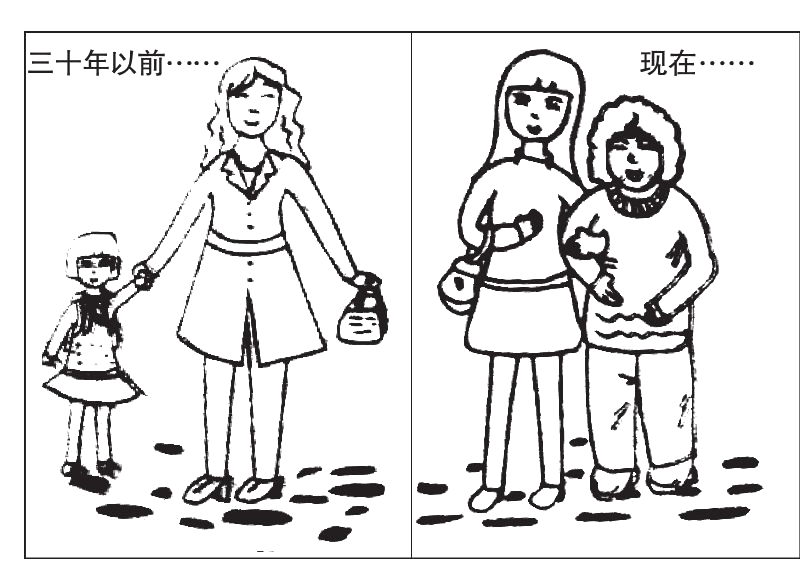
\includegraphics[width=0.56\linewidth]{picture/2014.png}
	\caption*{相携}
\end{figure}


